% LaTeX Curriculum Vitae Template
%
% Copyright (C) 2004-2009 Jason Blevins <jrblevin@sdf.lonestar.org>
% http://jblevins.org/projects/cv-template/
%
% You may use use this document as a template to create your own CV
% and you may redistribute the source code freely. No attribution is
% required in any resulting documents. I do ask that you please leave
% this notice and the above URL in the source code if you choose to
% redistribute this file.

\documentclass[letterpaper]{article}

\usepackage[SlantFont]{xeCJK}
%\setCJKmainfont{兰亭黑-简}
\setCJKmainfont[BoldFont=兰亭黑-简,ItalicFont=STKaiti]{STSong}
\usepackage{fontspec}
\setmainfont
  [ BoldFont   = HelveticaNeue-Bold.otf,
    ItalicFont = HelveticaNeue-LightItalic.otf ]
  {HelveticaNeue-Light.otf}
\setsansfont{HelveticaNeue-Light.otf}
% \setmonofont{Courier New}

\usepackage{hyperref}
\usepackage{geometry}

% Set your name here
\def\name{Qinglin Li}
% Chinese name here
\def\cname{李青林}

% Replace this with a link to your CV if you like, or set it empty
% (as in \def\footerlink{}) to remove the link in the footer:
\def\footerlink{}

% The following metadata will show up in the PDF properties
\hypersetup{
  colorlinks = true,
  urlcolor = black,
  pdfauthor = {\name},
  pdfkeywords = {computer science, machine learning},
  pdftitle = {\name: Curriculum Vitae},
  pdfsubject = {Curriculum Vitae},
  pdfpagemode = UseNone
}

\geometry{
  body={6.5in, 9.5in},
  left=0.8in,
  top=0.8in
}

% Customize page headers
\pagestyle{myheadings}
\markright{\name}
\thispagestyle{empty}

% Custom section fonts
\usepackage{sectsty}
\sectionfont{\large}

% Other possible font commands include:
% \ttfamily for teletype,
% \sffamily for sans serif,
% \bfseries for bold,
% \scshape for small caps,
% \normalsize, \large, \Large, \LARGE sizes.

% Don't indent paragraphs.
\setlength\parindent{0em}

\usepackage{wasysym}

\begin{document}

\begin{minipage}{0.35\linewidth}
  {\huge  \cname}
  \vspace{0.1in} \\
%  Born on June 1, 1993. Male. \\
  \href{http://www.sjtu.edu.cn/}{上海交通大学}
\end{minipage}
\begin{minipage}{0.45\linewidth}
  \begin{tabular}{ll}
    Gmail:  & \href{mailto:jack951753@gmail.com}{\tt jack951753@gmail.com} \\
    GitHub: & \href{https://github.com/lostleaf}{\tt http://github.com/lostleaf} \\
    Tel(Shanghai):    & {\tt +86 151-2112-7746}\\
    Tel(Beijing): & {\tt +86 131-4103-8926}
  \end{tabular}
\end{minipage}
\begin{minipage}{0.45\linewidth}
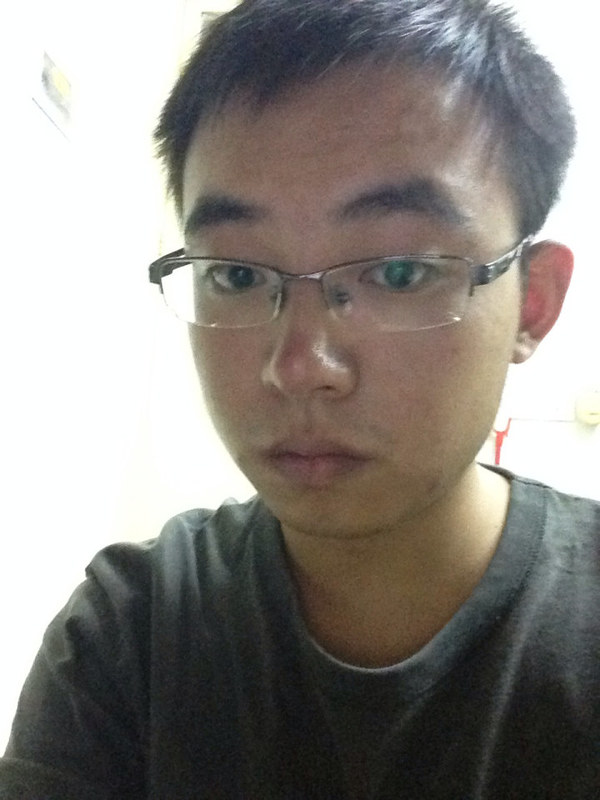
\includegraphics[width=40pt]{photo}
\end{minipage}

我是上海交通大学 \textbf{\href{http://acm.sjtu.edu.cn}{ACM班}} 的一名学生.我从 2003 年左右接触编程,目前能熟练使用多种编程语言和技术.我目前主要的研究领域为 \textbf{机器学习} 和 \textbf{计算视觉} .我对于 {\it Web开发} 和 {\it 数据分析} 也很有兴趣. 


\section*{教育背景}

\begin{itemize}

\item  本科,计算机科学专业.\quad\quad~2011.9 - 2015.6~(预计) \\
    \emph{\href{http://acm.sjtu.edu.cn}{ACM班},
    \href{http://www.sjtu.edu.cn/}{上海交通大学}.}
\end{itemize}

\section*{个人经历}
\begin{itemize}
\item \textbf{研究实习生} \emph{\href{http://research.microsoft.com/en-us/labs/asia/}{微软亚洲研究院}} ~\qquad\qquad\qquad\qquad2014.8 - 2015.2~(预计)\\
    导师:~~~~~~~~~~\emph{\href{http://bcmi.sjtu.edu.cn/~zhangliqing/}{李沐博士}}\\
    研究领域:~~~自然语言处理.
\item \textbf{研究助理} \emph{\href{http://bcmi.sjtu.edu.cn}{仿脑计算与机器智能研究中心}}\qquad\quad~~2013.7至今\\
    导师:~~~~~~~~~~\emph{\href{http://bcmi.sjtu.edu.cn/~zhangliqing/}{张丽清教授}}\\
    研究领域:~~~计算视觉.
\item \textbf{助教}  \emph{\href{http://acm.sjtu.edu.cn/wiki/Programming_2013}{C++ 程序设计}}\quad\qquad\qquad\qquad\qquad\quad\qquad~2013.9 - 2014.1\\
助教团队总负责人.
\end{itemize}
\section*{技能}
\begin{itemize}
\item 机器学习相关: Python, Matlab, C/C++.
\item Web开发相关: Ruby, Rails, HTML, javascript, CSS.
\item 桌面开发相关: Java.
\end{itemize}
\section*{部分项目经历 \normalsize{\it(\href{https://github.com/lostleaf?tab=repositories}{更多细节})}}
\begin{itemize}
\item \textbf{Crowd Density Estimation in Video}:
利用机器学习方法,估算公共场所中高密度高遮挡度场景下的人流密度,该项目入选上海市大学生创新项目.
\item \textbf{\href{http://acm.sjtu.edu.cn/ricsrt/}{Ranking Tool Research Capacity in CS}}:
在\textit{\href{http://www.cs.cornell.edu/jeh/}{John Hopcroft教授}}的指导下实现的一个项目, 用于衡量和比较计算机科学领域中不同国家和机构的研究生产力、质量和影响力,并且对结果进行了可视化.
\item \textbf{\href{https://github.com/lostleaf/compiler}{C Language Compiler}}:
使用 Java 实现的一个C语言编译器,支持 C语言 的大部分特性,并且以 MIPS 架构为编译目标,该项目完全实现了寄存器分配以及多种优化.
\item \textbf{\href{https://github.com/lostleaf/nachos}{Nachos Operating System}}: 
使用 Java 实现的一个模拟操作系统,功能包括多线程和多道编程、缓存和虚拟内存以及自己设计的文件系统文件系统等.
\item \textbf{\href{https://github.com/lostleaf/cpu}{Simulated CPU}}:
使用 Verilog 实现的一项模拟CPU,完全实现了 Tomasulo 算法,并模拟了缓存系统. 该CPU可以仿真执行 MIPS 汇编语言的一个图灵完备的子集.

\end{itemize}

\section*{获奖情况}
\begin{itemize}
\item  美国大学生数学建模竞赛\textbf{Honorable Mention(二等奖)}, 2014.
\item 中国大学生数学建模竞赛(CUMCM) \textbf{三等奖}, 2013. 
\item 全国信息学奥林匹克竞赛(NOI) \textbf{银牌}, 2010. 
\end{itemize}

\end{document}
